\documentclass[conference]{IEEEtran}
\usepackage{enumitem}
\usepackage{amsmath}
\usepackage{cite}
\usepackage{graphicx}
\graphicspath{ {./}{./images/} }

\title{PCA-Based Image Compression}

\author{
\IEEEauthorblockN{Owen Sowatzke}
\IEEEauthorblockA{\textit{Electrical Engineering Department} \\
\textit{University of Arizona}\\
Tucson, USA \\
osowatzke@arizona.edu}
\and
\IEEEauthorblockN{Scott Thoesen}
\IEEEauthorblockA{\textit{Electrical Engineering Department} \\
\textit{University of Arizona}\\
Tucson, USA \\
thoesens@arizona.edu}}

\begin{document}
    \maketitle
		
    \section{Introduction}
    This project aims to explore principle component analysis (PCA), its relationship to singular value decomposition (SVD), and its application to the field of image compression \cite{jaradet_svd_image_compression}. The topic of digital image compression has become more important than ever with the advent of smartphones and social media, with millions of images created, stored, transferred, and copied daily. Reducing the digital footprint of this data is therefore necessary to both satisfying end-user demands and decreasing the demand on limited computing and storage resources. Although image compression is interesting and generally important, it is not of particular importance to the authors. What is important to the authors is the more generalized use of PCA as a tool for data analysis and dimensionality reduction. Image compression was selected for this project to visually demonstrate the connection that is made by PCA between real-world data and linear algebra.

    \section{Background}
    PCA was not explicitly covered in ECE 501b but its underlying machinery, the SVD was. An entire lecture was dedicated to covering the SVD, which is an accumulation of many core concepts learned throughout the semester. The SVD employs many linear algebra concepts including inner product spaces, the null space, injectivity and surjectivity, dimensionality, linear independence, bases, orthonormality, linear maps, eigenvalues and eigenvectors, adjoints of linear maps, square roots of linear maps, matrix representations of linear maps, matrix decomposition, diagonal matrices, square matrices, unitary and orthonormal matrices.

    Motivation for compression of natural images?


    \subsection{Singular Value Decomposition}
    The Singular Value Decomposition Theorem states that for any matrix A (element of Fmxn), a unique representation of the form shown in equation (ref eq) exists [ref].

     \begin{equation*}{\mathbf{A}} = {\mathbf{U\Sigma }}{{\mathbf{V}}^{\mathbf{T}}}\tag{2}\end{equation*}

    where U(element of Fmxm) and V(element of Fnxn) are square unitary
    matrices whose columns represent the left singular vectors and right singular vectors, respectively, and Sigma(element of Fmxn) is a matrix of zeros except for the elements of the main diagonal which are called singular values. The singular values of A are always non-negative and real. When A is a real matrix, U and V are real and thus orthonormal.

    A literal interpretation of the SVD is the action taken by a linear map split into three discrete operations. The first operation performs a rotation of a vector onto an orthonormal basis in the domain of the map. The second operation simultaneously scales the vector and potentially changes dimensionality. The final operation is a rotation onto an orthonormal basis in the co-domain of the map.

    The SVD is a generalized analog of the eigendecomposition of a matrix, which is a result of the Spectral Theorem for certain linear operators, or square matrices (ref eigendecomp)(ref spectral). The eigenvectors of a full-rank normal operator, found through eigendecomposition, form an orthonormal basis on the inner product space of the operator called an eigenbasis. Thus, any vector in the inner product space can be represented completely and uniquely as an appropriate scaling of the eigenbasis vectors. The vectors of an eigenbasis are also called the modes of the operator. The magnitude of the eigenvalue associated with each mode determines the relative importance, or significance, of the mode. Modes with higher importance, or larger eigenvalues, contain more pertinent information about a vector than modes with smaller eigenvalues. In similar fashion, the right singular vectors of any operator represent the modes of the operator in the domain and the left singular vectors represent the modes in the co-domain. The magnitudes of the singular values determine the relative joint-importance, or joint-significance, of the associated singular vectors.
    
    \subsection{Principle Component Analysis} \label{pca_section}
    
    Using linear combinations of the existing basis, Principle Component Analysis (PCA) seeks to create a new basis which better represents the data \cite{shlens_2014_tutorial}. Let $\mathbf{X}$ be an mxn matrix of samples given with respect to the original basis, and let $\mathbf{Y}$ be an mxn matrix of samples given with respect to the updated basis. The operator $\mathbf{P}$ is an mxm matrix which re-expresses the samples in $\mathbf{X}$ in terms of an updated basis \cite{shlens_2014_tutorial}.
    
    \begin{equation}
    		\mathbf{Y} = \mathbf{PX}
    \end{equation}
    
    TALK ABOUT PCA HERE
    How does the selected material for your project relate to SVD?
    Theory of compression using PCA


    \section{Results}

    The compression technique described in Section \ref{pca_section} is implemented in Matlab. The Matlab built-in image 'wagon.jpg' is used throughout this section as an example for both qualitative and quantitative analysis of the compression scheme. Qualitative analysis is performed through visual inspection of image quality after compression. Quantitative analysis is performed by examining the peak signal-to-noise ratio (PSNR) of the compressed image, compared to the original, uncompressed image.

    \subsection{Data}
    Talk about image properties here, including size and format.

    \subsection{Design}
    Describe what the Matlab code is doing here. Talk about the color space conversion too.

    \subsection{Analysis}
    As mentioned in Section \ref{pca_section} every matrix can be decomposed into a linear combination of its principle components. The relative importance, or significance, of a principle component is determined by the magnitude of its associated singular value. A digital image is represented by a matrix and is therefore decomposed in the same way. In the context of image decomposition, the magnitude of each singular value determines the relative quantity of image information present in the respective principle components. Shown in Figure \ref{fig:svalplot} is a plot of all 768 singular values of the image wagon.jpg.

    \begin{figure}[t]
    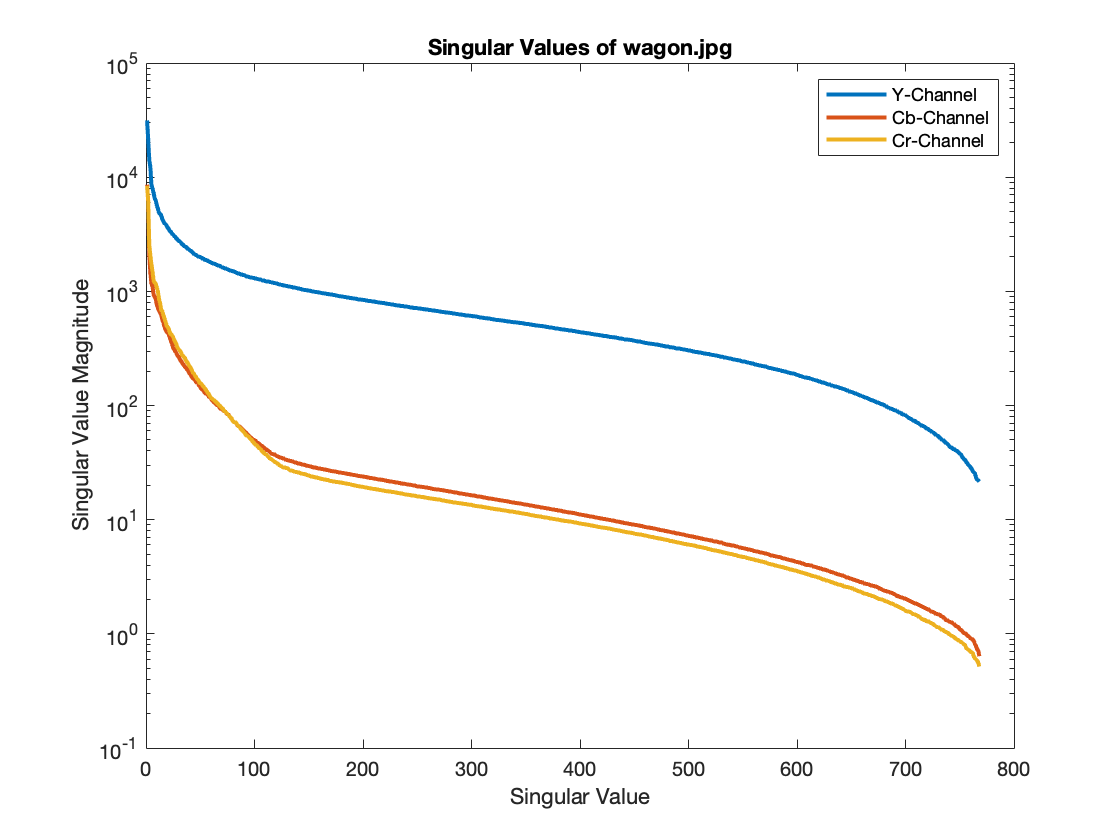
\includegraphics[width=0.5\textwidth]{svals_wagon}
    \caption{Plot showing the singular values of wagon.jpg. The SVD is computed separately for the luminance (Y), and both chrominance (Cb and Cr) channels}
    \label{fig:svalplot}
    \end{figure}
    
    
    Using the 25,000,000,000 Eigenvector paper as a guide, develop some exercises, questions, analysis, or examples that were inspired or motivated by your project. For example, what assumptions were made in your project material? What if certain assumptions are neglected or do not exist? Can you provide analysis that supplements the analysis in the selected project material Or, can you provide analysis that extends the analysis in the project material You might also develop numerical examples that help to provide insight into the ideas discussed in the selected material or that demonstrate the application of the theory in your project. The example you create might consist of a MATLAB simulation or MATLAB analysis.


    \section{Conclusion}
    
    Provide a summary and conclusion section in the report. How well did your example correlate or explain the concepts in the selected material? How would you modify your example to make it better? How did your selected project enhance your understanding of ECE 501b material?

    \nocite{jaradet_svd_image_compression}
    \nocite{shlens_2014_tutorial}
    \nocite{omar_image_compression}
    \nocite{xu_color_conversion}
    \newpage
    \bibliography{sources}{}
    \bibliographystyle{ieeetr}
\end{document}
